
%% bare_jrnl.tex
%% V1.4b
%% 2015/08/26
%% by Michael Shell
%% see http://www.michaelshell.org/
%% for current contact information.
%%
%% This is a skeleton file demonstrating the use of IEEEtran.cls
%% (requires IEEEtran.cls version 1.8b or later) with an IEEE
%% journal paper.
%%
%% Support sites:
%% http://www.michaelshell.org/tex/ieeetran/
%% http://www.ctan.org/pkg/ieeetran
%% and
%% http://www.ieee.org/

%%*************************************************************************
%% Legal Notice:
%% This code is offered as-is without any warranty either expressed or
%% implied; without even the implied warranty of MERCHANTABILITY or
%% FITNESS FOR A PARTICULAR PURPOSE! 
%% User assumes all risk.
%% In no event shall the IEEE or any contributor to this code be liable for
%% any damages or losses, including, but not limited to, incidental,
%% consequential, or any other damages, resulting from the use or misuse
%% of any information contained here.
%%
%% All comments are the opinions of their respective authors and are not
%% necessarily endorsed by the IEEE.
%%
%% This work is distributed under the LaTeX Project Public License (LPPL)
%% ( http://www.latex-project.org/ ) version 1.3, and may be freely used,
%% distributed and modified. A copy of the LPPL, version 1.3, is included
%% in the base LaTeX documentation of all distributions of LaTeX released
%% 2003/12/01 or later.
%% Retain all contribution notices and credits.
%% ** Modified files should be clearly indicated as such, including  **
%% ** renaming them and changing author support contact information. **
%%*************************************************************************


% *** Authors should verify (and, if needed, correct) their LaTeX system  ***
% *** with the testflow diagnostic prior to trusting their LaTeX platform ***
% *** with production work. The IEEE's font choices and paper sizes can   ***
% *** trigger bugs that do not appear when using other class files.       ***                          ***
% The testflow support page is at:
% http://www.michaelshell.org/tex/testflow/



\documentclass[journal]{IEEEtran}
\usepackage{float}
\usepackage[brazilian]{babel}
\usepackage[utf8]{inputenc}
\usepackage[T1]{fontenc}
\usepackage{graphicx,xcolor,enumerate}
\usepackage{url}
%
% If IEEEtran.cls has not been installed into the LaTeX system files,
% manually specify the path to it like:
% \documentclass[journal]{../sty/IEEEtran}





% Some very useful LaTeX packages include:
% (uncomment the ones you want to load)


% *** MISC UTILITY PACKAGES ***
%
%\usepackage{ifpdf}
% Heiko Oberdiek's ifpdf.sty is very useful if you need conditional
% compilation based on whether the output is pdf or dvi.
% usage:
% \ifpdf
%   % pdf code
% \else
%   % dvi code
% \fi
% The latest version of ifpdf.sty can be obtained from:
% http://www.ctan.org/pkg/ifpdf
% Also, note that IEEEtran.cls V1.7 and later provides a builtin
% \ifCLASSINFOpdf conditional that works the same way.
% When switching from latex to pdflatex and vice-versa, the compiler may
% have to be run twice to clear warning/error messages.






% *** CITATION PACKAGES ***
%
%\usepackage{cite}
% cite.sty was written by Donald Arseneau
% V1.6 and later of IEEEtran pre-defines the format of the cite.sty package
% \cite{} output to follow that of the IEEE. Loading the cite package will
% result in citation numbers being automatically sorted and properly
% "compressed/ranged". e.g., [1], [9], [2], [7], [5], [6] without using
% cite.sty will become [1], [2], [5]--[7], [9] using cite.sty. cite.sty's
% \cite will automatically add leading space, if needed. Use cite.sty's
% noadjust option (cite.sty V3.8 and later) if you want to turn this off
% such as if a citation ever needs to be enclosed in parenthesis.
% cite.sty is already installed on most LaTeX systems. Be sure and use
% version 5.0 (2009-03-20) and later if using hyperref.sty.
% The latest version can be obtained at: 

% http://www.ctan.org/pkg/cite
% The documentation is contained in the cite.sty file itself.






% *** GRAPHICS RELATED PACKAGES ***
%
\ifCLASSINFOpdf
  % \usepackage[pdftex]{graphicx}
  % declare the path(s) where your graphic files are
  % \graphicspath{{../pdf/}{../jpeg/}}
  % and their extensions so you won't have to specify these with
  % every instance of \includegraphics
  % \DeclareGraphicsExtensions{.pdf,.jpeg,.png}
\else
  % or other class option (dvipsone, dvipdf, if not using dvips). graphicx
  % will default to the driver specified in the system graphics.cfg if no
  % driver is specified.
  % \usepackage[dvips]{graphicx}
  % declare the path(s) where your graphic files are
  % \graphicspath{{../eps/}}
  % and their extensions so you won't have to specify these with
  % every instance of \includegraphics
  % \DeclareGraphicsExtensions{.eps}
\fi
% graphicx was written by David Carlisle and Sebastian Rahtz. It is
% required if you want graphics, photos, etc. graphicx.sty is already
% installed on most LaTeX systems. The latest version and documentation
% can be obtained at: 
% http://www.ctan.org/pkg/graphicx
% Another good source of documentation is "Using Imported Graphics in
% LaTeX2e" by Keith Reckdahl which can be found at:
% http://www.ctan.org/pkg/epslatex
%
% latex, and pdflatex in dvi mode, support graphics in encapsulated
% postscript (.eps) format. pdflatex in pdf mode supports graphics
% in .pdf, .jpeg, .png and .mps (metapost) formats. Users should ensure
% that all non-photo figures use a vector format (.eps, .pdf, .mps) and
% not a bitmapped formats (.jpeg, .png). The IEEE frowns on bitmapped formats
% which can result in "jaggedy"/blurry rendering of lines and letters as
% well as large increases in file sizes.
%
% You can find documentation about the pdfTeX application at:
% http://www.tug.org/applications/pdftex





% *** MATH PACKAGES ***
%
%\usepackage{amsmath}
% A popular package from the American Mathematical Society that provides
% many useful and powerful commands for dealing with mathematics.
%
% Note that the amsmath package sets \interdisplaylinepenalty to 10000
% thus preventing page breaks from occurring within multiline equations. Use:
%\interdisplaylinepenalty=2500
% after loading amsmath to restore such page breaks as IEEEtran.cls normally
% does. amsmath.sty is already installed on most LaTeX systems. The latest
% version and documentation can be obtained at:
% http://www.ctan.org/pkg/amsmath





% *** SPECIALIZED LIST PACKAGES ***
%
%\usepackage{algorithmic}
% algorithmic.sty was written by Peter Williams and Rogerio Brito.
% This package provides an algorithmic environment fo describing algorithms.
% You can use the algorithmic environment in-text or within a figure
% environment to provide for a floating algorithm. Do NOT use the algorithm
% floating environment provided by algorithm.sty (by the same authors) or
% algorithm2e.sty (by Christophe Fiorio) as the IEEE does not use dedicated
% algorithm float types and packages that provide these will not provide
% correct IEEE style captions. The latest version and documentation of
% algorithmic.sty can be obtained at:
% http://www.ctan.org/pkg/algorithms
% Also of interest may be the (relatively newer and more customizable)
% algorithmicx.sty package by Szasz Janos:
% http://www.ctan.org/pkg/algorithmicx




% *** ALIGNMENT PACKAGES ***
%
%\usepackage{array}
% Frank Mittelbach's and David Carlisle's array.sty patches and improves
% the standard LaTeX2e array and tabular environments to provide better
% appearance and additional user controls. As the default LaTeX2e table
% generation code is lacking to the point of almost being broken with
% respect to the quality of the end results, all users are strongly
% advised to use an enhanced (at the very least that provided by array.sty)
% set of table tools. array.sty is already installed on most systems. The
% latest version and documentation can be obtained at:
% http://www.ctan.org/pkg/array


% IEEEtran contains the IEEEeqnarray family of commands that can be used to
% generate multiline equations as well as matrices, tables, etc., of high
% quality.




% *** SUBFIGURE PACKAGES ***
%\ifCLASSOPTIONcompsoc
%  \usepackage[caption=false,font=normalsize,labelfont=sf,textfont=sf]{subfig}
%\else
%  \usepackage[caption=false,font=footnotesize]{subfig}
%\fi
% subfig.sty, written by Steven Douglas Cochran, is the modern replacement
% for subfigure.sty, the latter of which is no longer maintained and is
% incompatible with some LaTeX packages including fixltx2e. However,
% subfig.sty requires and automatically loads Axel Sommerfeldt's caption.sty
% which will override IEEEtran.cls' handling of captions and this will result
% in non-IEEE style figure/table captions. To prevent this problem, be sure
% and invoke subfig.sty's "caption=false" package option (available since
% subfig.sty version 1.3, 2005/06/28) as this is will preserve IEEEtran.cls
% handling of captions.
% Note that the Computer Society format requires a larger sans serif font
% than the serif footnote size font used in traditional IEEE formatting
% and thus the need to invoke different subfig.sty package options depending
% on whether compsoc mode has been enabled.
%
% The latest version and documentation of subfig.sty can be obtained at:
% http://www.ctan.org/pkg/subfig




% *** FLOAT PACKAGES ***
%
%\usepackage{fixltx2e}
% fixltx2e, the successor to the earlier fix2col.sty, was written by
% Frank Mittelbach and David Carlisle. This package corrects a few problems
% in the LaTeX2e kernel, the most notable of which is that in current
% LaTeX2e releases, the ordering of single and double column floats is not
% guaranteed to be preserved. Thus, an unpatched LaTeX2e can allow a
% single column figure to be placed prior to an earlier double column
% figure.
% Be aware that LaTeX2e kernels dated 2015 and later have fixltx2e.sty's
% corrections already built into the system in which case a warning will
% be issued if an attempt is made to load fixltx2e.sty as it is no longer
% needed.
% The latest version and documentation can be found at:
% http://www.ctan.org/pkg/fixltx2e


%\usepackage{stfloats}
% stfloats.sty was written by Sigitas Tolusis. This package gives LaTeX2e
% the ability to do double column floats at the bottom of the page as well
% as the top. (e.g., "\begin{figure*}[!b]" is not normally possible in
% LaTeX2e). It also provides a command:
%\fnbelowfloat
% to enable the placement of footnotes below bottom floats (the standard
% LaTeX2e kernel puts them above bottom floats). This is an invasive package
% which rewrites many portions of the LaTeX2e float routines. It may not work
% with other packages that modify the LaTeX2e float routines. The latest
% version and documentation can be obtained at:
% http://www.ctan.org/pkg/stfloats
% Do not use the stfloats baselinefloat ability as the IEEE does not allow
% \baselineskip to stretch. Authors submitting work to the IEEE should note
% that the IEEE rarely uses double column equations and that authors should try
% to avoid such use. Do not be tempted to use the cuted.sty or midfloat.sty
% packages (also by Sigitas Tolusis) as the IEEE does not format its papers in
% such ways.
% Do not attempt to use stfloats with fixltx2e as they are incompatible.
% Instead, use Morten Hogholm'a dblfloatfix which combines the features
% of both fixltx2e and stfloats:
%
% \usepackage{dblfloatfix}
% The latest version can be found at:
% http://www.ctan.org/pkg/dblfloatfix




%\ifCLASSOPTIONcaptionsoff
%  \usepackage[nomarkers]{endfloat}
% \let\MYoriglatexcaption\caption
% \renewcommand{\caption}[2][\relax]{\MYoriglatexcaption[#2]{#2}}
%\fi
% endfloat.sty was written by James Darrell McCauley, Jeff Goldberg and 
% Axel Sommerfeldt. This package may be useful when used in conjunction with 
% IEEEtran.cls'  captionsoff option. Some IEEE journals/societies require that
% submissions have lists of figures/tables at the end of the paper and that
% figures/tables without any captions are placed on a page by themselves at
% the end of the document. If needed, the draftcls IEEEtran class option or
% \CLASSINPUTbaselinestretch interface can be used to increase the line
% spacing as well. Be sure and use the nomarkers option of endfloat to
% prevent endfloat from "marking" where the figures would have been placed
% in the text. The two hack lines of code above are a slight modification of
% that suggested by in the endfloat docs (section 8.4.1) to ensure that
% the full captions always appear in the list of figures/tables - even if
% the user used the short optional argument of \caption[]{}.
% IEEE papers do not typically make use of \caption[]'s optional argument,
% so this should not be an issue. A similar trick can be used to disable
% captions of packages such as subfig.sty that lack options to turn off
% the subcaptions:
% For subfig.sty:
% \let\MYorigsubfloat\subfloat
% \renewcommand{\subfloat}[2][\relax]{\MYorigsubfloat[]{#2}}
% However, the above trick will not work if both optional arguments of
% the \subfloat command are used. Furthermore, there needs to be a
% description of each subfigure *somewhere* and endfloat does not add
% subfigure captions to its list of figures. Thus, the best approach is to
% avoid the use of subfigure captions (many IEEE journals avoid them anyway)
% and instead reference/explain all the subfigures within the main caption.
% The latest version of endfloat.sty and its documentation can obtained at:
% http://www.ctan.org/pkg/endfloat
%
% The IEEEtran \ifCLASSOPTIONcaptionsoff conditional can also be used
% later in the document, say, to conditionally put the References on a 
% page by themselves.




% *** PDF, URL AND HYPERLINK PACKAGES ***
%
%\usepackage{url}
% url.sty was written by Donald Arseneau. It provides better support for
% handling and breaking URLs. url.sty is already installed on most LaTeX
% systems. The latest version and documentation can be obtained at:
% http://www.ctan.org/pkg/url
% Basically, \url{my_url_here}.




% *** Do not adjust lengths that control margins, column widths, etc. ***
% *** Do not use packages that alter fonts (such as pslatex).         ***
% There should be no need to do such things with IEEEtran.cls V1.6 and later.
% (Unless specifically asked to do so by the journal or conference you plan
% to submit to, of course. )


% correct bad hyphenation here
\hyphenation{op-tical net-works semi-conduc-tor}


\begin{document}
%
% paper title
% Titles are generally capitalized except for words such as a, an, and, as,
% at, but, by, for, in, nor, of, on, or, the, to and up, which are usually
% not capitalized unless they are the first or last word of the title.
% Linebreaks \\ can be used within to get better formatting as desired.
% Do not put math or special symbols in the title.
\title{Processador com dois núcleos\\ com ambos superescalares}
%
%
% author names and IEEE memberships
% note positions of commas and nonbreaking spaces ( ~ ) LaTeX will not break
% a structure at a ~ so this keeps an author's name from being broken across
% two lines.
% use \thanks{} to gain access to the first footnote area
% a separate \thanks must be used for each paragraph as LaTeX2e's \thanks
% was not built to handle multiple paragraphs
%

\author{Gabriel~T.~H.~Santos~RA:107774, Thiago~I.~Yasunaka~RA:103069~}

% note the % following the last \IEEEmembership and also \thanks - 
% these prevent an unwanted space from occurring between the last author name
% and the end of the author line. i.e., if you had this:
% 
% \author{....lastname \thanks{...} \thanks{...} }
%                     ^------------^------------^----Do not want these spaces!
%
% a space would be appended to the last name and could cause every name on that
% line to be shifted left slightly. This is one of those "LaTeX things". For
% instance, "\textbf{A} \textbf{B}" will typeset as "A B" not "AB". To get
% "AB" then you have to do: "\textbf{A}\textbf{B}"
% \thanks is no different in this regard, so shield the last } of each \thanks
% that ends a line with a % and do not let a space in before the next \thanks.
% Spaces after \IEEEmembership other than the last one are OK (and needed) as
% you are supposed to have spaces between the names. For what it is worth,
% this is a minor point as most people would not even notice if the said evil
% space somehow managed to creep in.



% The paper headers
\markboth{Projeto III - Arquitetura de computadores II, Universidade Estadual de Maringá, Dezembro de 2020}%
{Shell \MakeLowercase{\textit{et al.}}: Processador com dois núcleos - com ambos superescalares}
% The only time the second header will appear is for the odd numbered pages
% after the title page when using the twoside option.
% 
% *** Note that you probably will NOT want to include the author's ***
% *** name in the headers of peer review papers.                   ***
% You can use \ifCLASSOPTIONpeerreview for conditional compilation here if
% you desire.




% If you want to put a publisher's ID mark on the page you can do it like
% this:
%\IEEEpubid{0000--0000/00\$00.00~\copyright~2015 IEEE}
% Remember, if you use this you must call \IEEEpubidadjcol in the second
% column for its text to clear the IEEEpubid mark.



% use for special paper notices
%\IEEEspecialpapernotice{(Invited Paper)}




% make the title area
\maketitle

% As a general rule, do not put math, special symbols or citations
% in the abstract or keywords.
\begin{abstract}
Em uma execução de pipeline o desempenho e efetividade são muito valorizados e para isto há vários estudos para ocorrer estes aprimoramentos, para isto um dos quais já são usados é o método de \textit{scoreboarding}, tal método será abordado neste projeto, juntamente com a utilização de \textit{threads}. A técnica de \textit{scoreboarding} consiste em um escalonador dinâmico de instruções que permite executar fora de ordem cada instrução desde que exista recursos disponíveis e que não haja dependência de dados. Além do \textit{scoreboarding}, haverá também a implementação de um simulador de \textit{threads} em um processador, que são alternativas para melhorar o desempenho dele. De forma simples, as \textit{threads} funcionam como um processo de execução concorrente, isto é, a capacidade do processador executar diversos processos de forma simultânea, podendo ou não ter memória compartilhada entre eles. 
\end{abstract}

% For peer review papers, you can put extra information on the cover
% page as needed:
% \ifCLASSOPTIONpeerreview
% \begin{center} \bfseries EDICS Category: 3-BBND \end{center}
% \fi
%
% For peerreview papers, this IEEEtran command inserts a page break and
% creates the second title. It will be ignored for other modes.
\IEEEpeerreviewmaketitle

\section{Introdução}
% The very first letter is a 2 line initial drop letter followed
% by the rest of the first word in caps.
% 
% form to use if the first word consists of a single letter:
% \IEEEPARstart{A}{demo} file is ....
% 
% form to use if you need the single drop letter followed by
% normal text (unknown if ever used by the IEEE):
% \IEEEPARstart{A}{}demo file is ....
% 
% Some journals put the first two words in caps:
% \IEEEPARstart{T}{his demo} file is ....
% 
% Here we have the typical use of a "T" for an initial drop letter
% and "HIS" in caps to complete the first word.
\IEEEPARstart {E}{ste} projeto baseia-se na implementação de um simulador da técnica de \textit{scoreboarding} em um processador de dois núcleos, simulando de forma completa os status de cada componente presente nela e em cada ciclo de \textit{clock}. O \textit{scoreboarding} foi usado pela primeira vez no computador \textit{CDC 6600} com o objetivo de organizar dinamicamente um \textit{pipeline} e consequentemente, melhorar o desempenho de um processador. No entanto, neste modelo proposto, a execução fora de ordem das instruções acabaram sendo frequentes. Para que não tenha conflito de dados, o \textit{scoreboarding} verifica minuciosamente cada etapa da sua execução antes de prosseguir para o próximo ciclo de \textit{clock}.

Com o intuito de melhorar ainda mais o desempenho de um processador, foi estudado uma maneira de executar diversos processos simultaneamente, dessa forma, o processador seria capaz de realizar operações de forma concorrente, podendo ou não compartilhar a mesma memórias entre eles. A proposta feita foi a criação de \textit{threads}, como foi dito acima, ela permite executar várias tarefas simultaneamente. De maneira informal, é como se existissem vários processadores dentro de um único processador. 
 
\hfill 10 de Dezembro de 2020

% An example of a floating figure using the graphicx package.
% Note that \label must occur AFTER (or within) \caption.
% For figures, \caption should occur after the \includegraphics.
% Note that IEEEtran v1.7 and later has special internal code that
% is designed to preserve the operation of \label within \caption
% even when the captionsoff option is in effect. However, because
% of issues like this, it may be the safest practice to put all your
% \label just after \caption rather than within \caption{}.
%
% Reminder: the "draftcls" or "draftclsnofoot", not "draft", class
% option should be used if it is desired that the figures are to be
% displayed while in draft mode.
%
%\begin{figure}[!t]
%\centering
%\includegraphics[width=2.5in]{myfigure}
% where an .eps filename suffix will be assumed under latex, 
% and a .pdf suffix will be assumed for pdflatex; or what has been declared
% via \DeclareGraphicsExtensions.
%\caption{Simulation results for the network.}
%\label{fig_sim}
%\end{figure}

% Note that the IEEE typically puts floats only at the top, even when this
% results in a large percentage of a column being occupied by floats.


% An example of a double column floating figure using two subfigures.
% (The subfig.sty package must be loaded for this to work.)
% The subfigure \label commands are set within each subfloat command,
% and the \label for the overall figure must come after \caption.
% \hfil is used as a separator to get equal spacing.
% Watch out that the combined width of all the subfigures on a 
% line do not exceed the text width or a line break will occur.
%
%\begin{figure*}[!t]
%\centering
%\subfloat[Case I]{\includegraphics[width=2.5in]{box}%
%\label{fig_first_case}}
%\hfil
%\subfloat[Case II]{\includegraphics[width=2.5in]{box}%
%\label{fig_second_case}}
%\caption{Simulation results for the network.}
%\label{fig_sim}
%\end{figure*}
%
% Note that often IEEE papers with subfigures do not employ subfigure
% captions (using the optional argument to \subfloat[]), but instead will
% reference/describe all of them (a), (b), etc., within the main caption.
% Be aware that for subfig.sty to generate the (a), (b), etc., subfigure
% labels, the optional argument to \subfloat must be present. If a
% subcaption is not desired, just leave its contents blank,
% e.g., \subfloat[].


% An example of a floating table. Note that, for IEEE style tables, the
% \caption command should come BEFORE the table and, given that table
% captions serve much like titles, are usually capitalized except for words
% such as a, an, and, as, at, but, by, for, in, nor, of, on, or, the, to
% and up, which are usually not capitalized unless they are the first or
% last word of the caption. Table text will default to \footnotesize as
% the IEEE normally uses this smaller font for tables.
% The \label must come after \caption as always.
%
%\begin{table}[!t]
%% increase table row spacing, adjust to taste
%\renewcommand{\arraystretch}{1.3}
% if using array.sty, it might be a good idea to tweak the value of
% \extrarowheight as needed to properly center the text within the cells
%\caption{An Example of a Table}
%\label{table_example}
%\centering
%% Some packages, such as MDW tools, offer better commands for making tables
%% than the plain LaTeX2e tabular which is used here.
%\begin{tabular}{|c||c|}
%\hline
%One & Two\\
%\hline
%Three & Four\\
%\hline
%\end{tabular}
%\end{table}


% Note that the IEEE does not put floats in the very first column
% - or typically anywhere on the first page for that matter. Also,
% in-text middle ("here") positioning is typically not used, but it
% is allowed and encouraged for Computer Society conferences (but
% not Computer Society journals). Most IEEE journals/conferences use
% top floats exclusively. 
% Note that, LaTeX2e, unlike IEEE journals/conferences, places
% footnotes above bottom floats. This can be corrected via the
% \fnbelowfloat command of the stfloats package.

\section{Scoreboarding}
Para o processamento, existem alguns pré-requisitos que foram definidos antes da implementação, as figuras 1 e 2 representam a arquitetura do \textit{scoreboarding} que será seguido, sendo mais detalhada sobre os processos que ocorre internamente na figura 2. Portanto, para o \textit{scoreboarding} temos quatro etapas importantes para o caminho desde a instrução até a escrita no registrador, das quais são listadas abaixo: 
\begin{itemize}
    \item Emissão \textit{(Issue)}
    \item Leitura de Operandos \textit{(Read Operand)}
    \item Execução \textit{(Execution)}
    \item Escrita dos Resultados \textit{(Write Results)}
\end{itemize}
A implementação abordará apenas instruções inteiras, diante disso teremos apenas estas unidades funcionais (UF): 
\begin{itemize}
    \item \textit{1 UF para soma/subtração}
    \item \textit{2 UF para multiplicação}
    \item \textit{1 UF para divisão}
    \item \textit{1 UF para operações lógicas}
\end{itemize}


\begin{center}
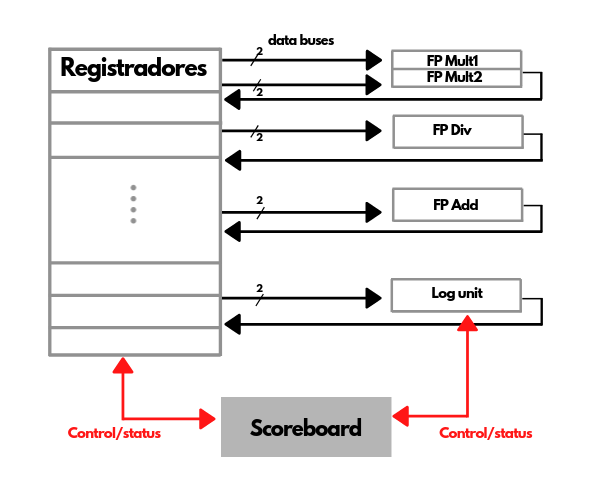
\includegraphics[scale=0.4]{img_Scoreboard.png}\\
\textbf{Figura 1:} Arquitetura \textit{Scoreboarding}
\end{center}

\begin{center}
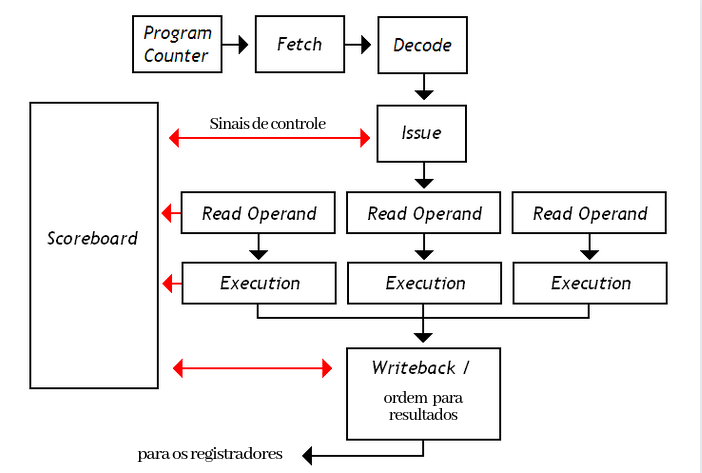
\includegraphics[scale=0.4]{img_Scoreboarding.png}\\
\textbf{Figura 2:} Arquitetura detalhada do \textit{Scoreboarding}
\end{center}

\section{Arquitetura Implementada}
Pode ser visto a seguir, na figura 3, a representação do diagrama da arquitetura a ser seguida neste projeto para a implementação já com o processador de dois núcleos.
\begin{center}
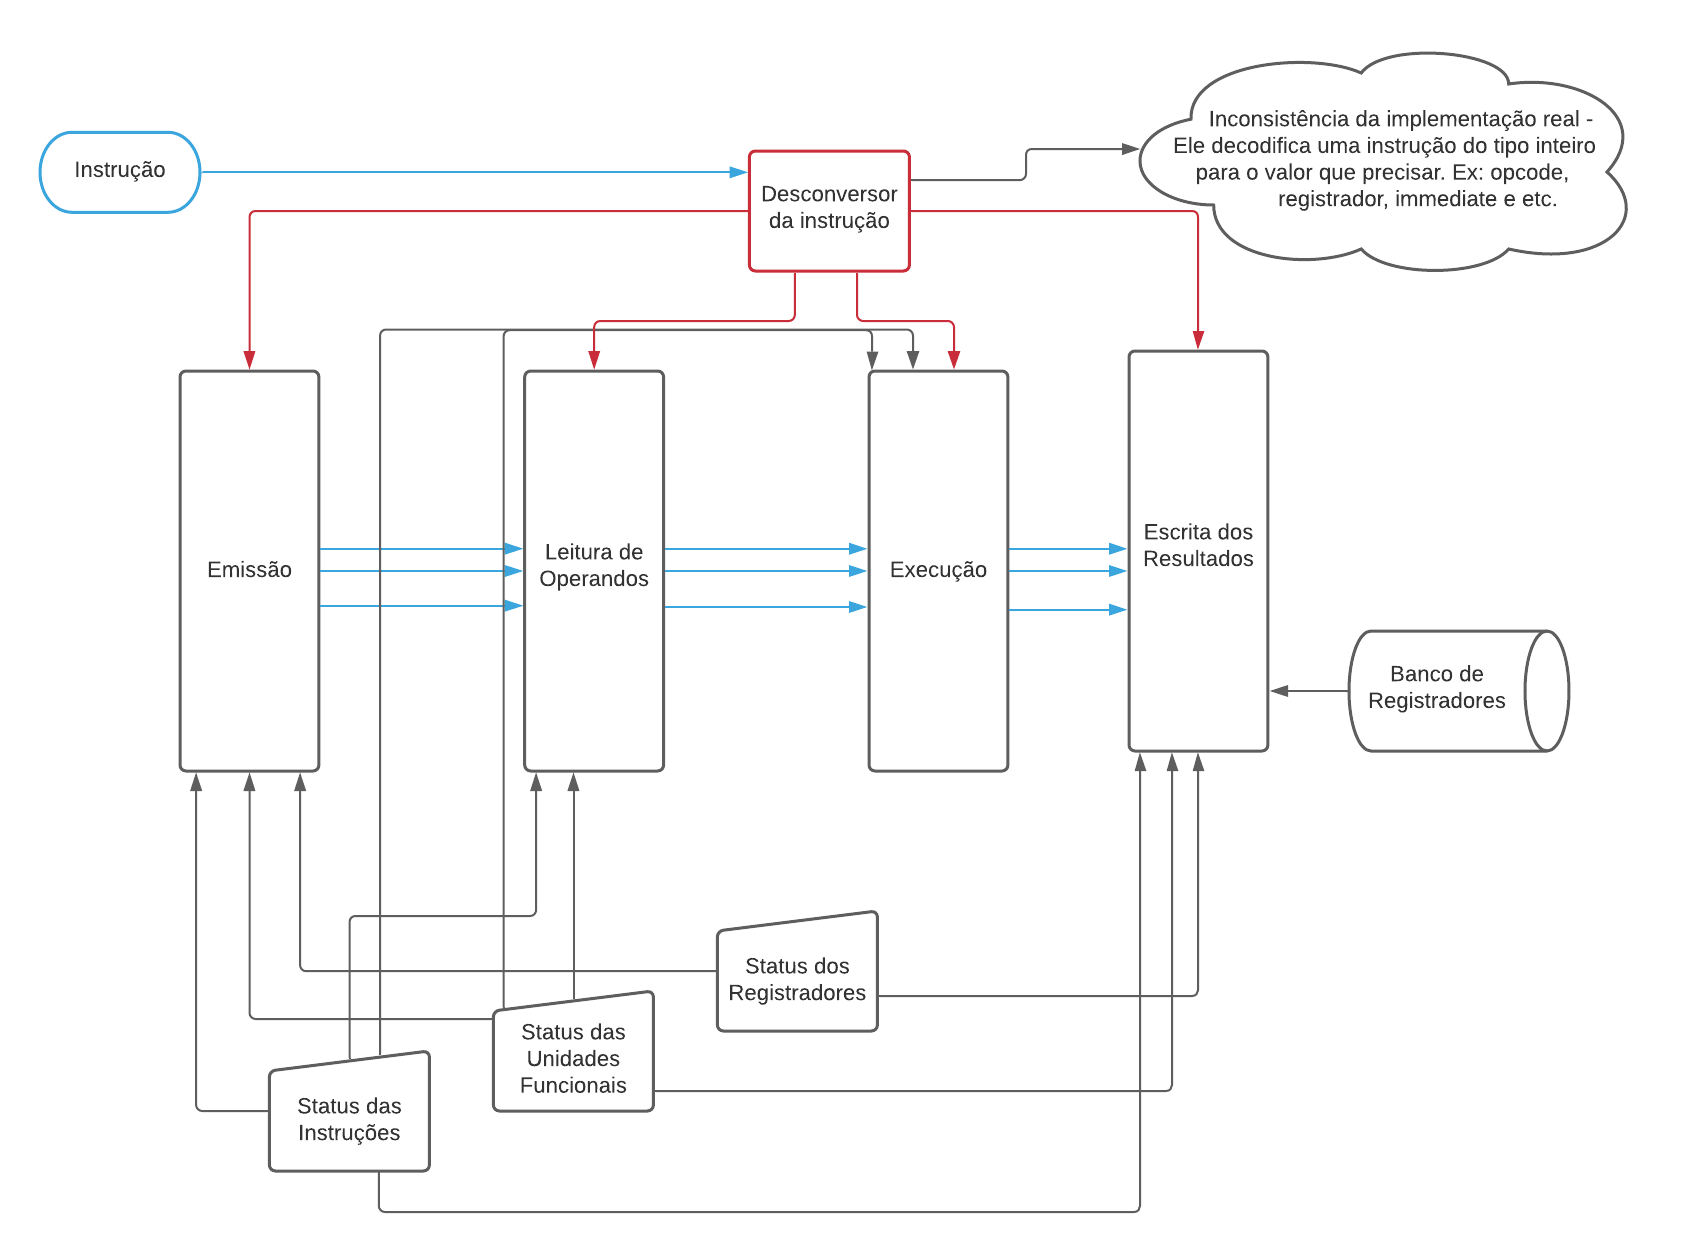
\includegraphics[scale=0.16]{arquitetura_implementada.png}\\
\textbf{Figura 3:} Arquitetura Implementada
\end{center}

Analisando a figura 3, observa-se que existem algumas inconsistências em relação a verdadeira implementação de um \textit{scoreboarding}, é fácil observar que existe um componente destacado em vermelho chamado "desconversor da instrução". Este item no diagrama faz a desconversão de uma instrução (representado por um número inteiro, ou seja, utilizando 32 \textit{bits})  para qualquer parâmetro que ela necessitar. Suponha que exista uma instrução \texttt{addi \$s1 \$s0 10}, utilizando este desconversor é possível resgatar qualquer um dos quatro parâmetros desta instrução, para isso basta utilizar uma função específica para realizar a operação. Um meio para contornar esta divergência, porem não abordado seria executar as operações de forma invertida, ou seja, da escrita dos resultados para a emissão, juntamente com \textit{structs} auxiliares.

A arquitetura consiste em quatro etapas principais: Emissão, leitura de operandos, execução e escrita dos resultados. Além destas quatro etapas necessárias para a simulação do \textit{scoreboarding}, é preciso outros quatro componentes que controlam os estados das instruções e dos registradores, para isso foi definido diversas \textit{structs} (escritas em linguagem C) que representam elas, sendo: status das instruções, status das unidades funcionais, status dos registradores e o banco de registradores, este último utilizado para armazenar os valores que cada registrador possui.

A figura 3 representa o processamento que apenas um núcleo do processador faz, porém, o projeto final trabalha com dois núcleos de processamento simultâneos. Para isso, utilizou-se a biblioteca em C chamada \textit{pthreads}, com ela é possível executar diversos fluxos de códigos de forma paralela, por exemplo, executar mais de uma função ao mesmo tempo. A figura 4 abaixo mostra um diagrama visual para exemplificar um processador utilizando dois núcleos com \textit{scoreboarding} implementado.

\begin{center}
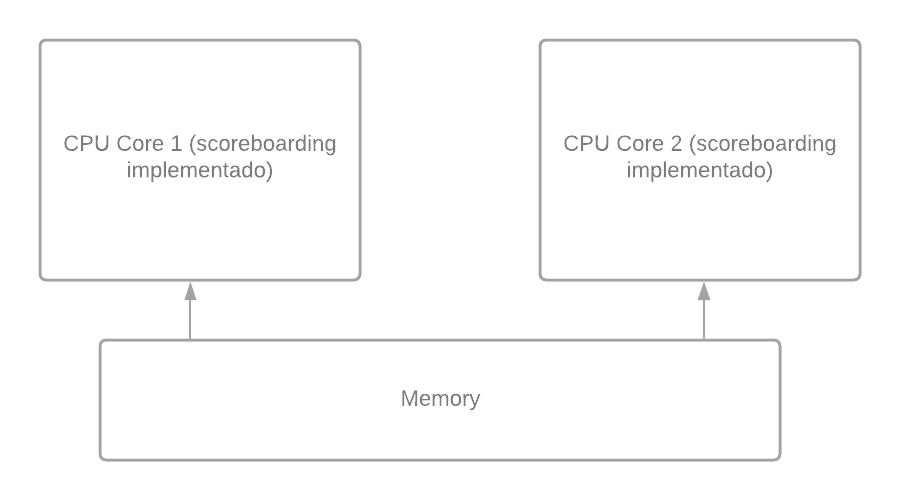
\includegraphics[scale=0.25]{threads.png}\\
\textbf{Figura 4:} Arquitetura com dois núcleos
\end{center}

A figura 4 mostra uma arquitetura desenvolvida com dois núcleos, por sua vez, estes núcleos são interligados por uma memória compartilhada. Como dito acima, a implementação das \textit{threads} foi codificada utilizando a biblioteca \textit{pthread} na linguagem C, o que representaria essa memória compartilhada no código seriam as variáveis globais. As variáveis globais no programa implementado são somente as variáveis recebidas por parâmetros, sendo elas: caminho para o arquivo de configuração, caminho dos programas 1 e 2, arquivo de saída para os programas 1 e 2 e a quantidade de instruções para os programas 1 e 2.

A ideia por trás de simular dois núcleos simultaneamente são definidos logo que o programa inicia. A partir dos parâmetros recebidos ocorrem a validação deles e após isso é chamado uma função \texttt{execute\_pthread} em que será responsável para as execuções seguintes, logo então é criado dois fluxos utilizando a função \texttt{pthread\_create()}, nela são passados os argumentos necessários e a função a ser executada, no caso, a execução do \textit{scoreboarding}. O fim da execução das \textit{threads} é realizado pela função \texttt{pthread\_join()}.

\section{Uma solução}
A inicialização do \textit{scoreboarding} ocorre a partir do arquivo \textit{pthreads.c}, nela são introduzidas as criações das \textit{threads} para a execução concorrente e além disso, durante a inicialização é organizado toda a configuração e início da execução do \textit{pipeline}.\\
A partir disso, referencia-se para chamada do processador (\textit{processador.c}), onde ficará a execução do escalonador e criação de todo o fluxo do \textit{scoreboarding}.\\
Para a implementação na linguagem \textit{C}, foram definidos \textit{structs} bases para cada etapa da arquitetura, isto quer dizer que cada componente do \textit{scoreboarding} recebeu uma estrutura própria para melhor representá-la. Foram estas \textit{structs}:
\begin{itemize}
    \item \textit{functional\_unit\_status\_table}
    \item \textit{instruction\_status\_linked}  
    \item \textit{register\_database}
    \item \textit{register\_result\_status\_table}
    \item \textit{config}
    \item \textit{I}, \textit{R}  
\end{itemize}.
A organização arquitetural utilizada dentro da execução do processador foi definida em separar-se em quatro funções principais, sendo elas nomeadas com a mesma nomenclatura das quatro etapas presentes no \textit{scoreboarding}. Por sua vez, por meio de passagem de parâmetros por referência, cada uma destas funções trabalha e implementa a lógica das execuções do \textit{scoreboarding} separadamente.
Durante o desenvolvimento foram utilizadas diversas funções auxiliares que foram armazenadas dentro do diretório \textit{/utils}, neste diretório existem funções que são utilizadas mais de uma vez. Este modelo foi necessário a fim de organização e remoção de código duplicado. Existem funções reutilizadas em outros arquivos também, como no caso do \textit{get's} e \textit{set's} nos arquivos do diretório \textit{/components} do projeto.
Um resumo da organização do projeto é definido na lista abaixo:
\begin{itemize}
    \item \textit{/components}: Definição das tabelas presentes no \textit{scoreboarding} e as unidades(\textit{mult1, mult2, add, log, divide}) que ela possui, sendo utilizado também um \textit{empty} para representar a não utilização.
    \item \textit{/config}: Integração com o arquivo de configuração que é recebido por parâmetro para a memória.  
    \item \textit{/examples}: Exemplos utilizados para os testes durante o desenvolvimento,
    \item \textit{/operations}: Implementação das operações que o MIPS (de acordo com a documentação do projeto) realiza e integração com o banco de registradores.
    \item \textit{/prints}: \textit{Prints} para a escrita no arquivo de saída para cada \textit{clock} e também análise dos dados resultantes. 
    \item \textit{/types}: Tipagem e definição das constantes a ser utilizado no projeto como um todo, por exemplo: Registradores, operações (\textit{addi}, \textit{add}, \textit{sub}, \textit{div},  \textit{etc.}) e tipos. Os valores das constantes seguiu a documentação oficial do \textit{greencard} do \textit{MIPS}, salvo as exceções para as operações LI e MOVE, que receberam os valores 28 e 30, e do tipo I e R, ambos respectivamente.
    \item \textit{/utils}: Este diretório contém diversas funções auxiliares que foram utilizados em todo o projeto, necessário para evitar possíveis duplicações de código.
    \item \textit{conversor.h}: Faz todas as conversões e desconversões necessárias para o conjunto de instruções e atribui à memória do programa.
    \item \textit{main.c}:  Verifica os parametros passados, caso haja algum de modo incorreto há o retorno e a não continuação do programa, caso contrario, aqui também se faz a chamada da execução das \textit{threads} e então a partir dele, como já comentado, o \textit{scoreboarding}.
    \item \textit{processador.c}: O \textit{scoreboarding} e toda a sua implementação depende desse arquivo. Aqui é implementado toda a lógica necessária, as inicializações dos componentes necessários para a simulação do \textit{scoreboarding}, principalmente por causa das \textit{threads}, houve a necessidade de se implementar ao mesmo arquivo. Como também grande parte das funções auxiliares são utilizadas em funções que pertencem a este arquivo. Sendo as suas principais funções de cada etapa da arquitetura (\textit{executeIssue()}, \textit{readOperands()}, \textit{executeOperands()}, \textit{writeResult()}) desenvolvidas dentro de um laço de repetição \textit{while} para simular as operações enquanto não há o término de todas as escritas de resultado. 
\end{itemize}.

\section{Análise e Discussão}

Para validar a implementação do simulador de \textit{scoreboarding} com a integração das \textit{threads}, foram executadas diversos testes no decorrer do desenvolvimento por etapas e também por funções, utilizando também \textit{debugger} para ver de fato quais e onde cada campo estava sendo modificado. A partir disso, foram criadas arquivos para o conjunto de instruções, com \textit{mnemonios} com base no material visto em aula e também pela \textit{internet} para confirmar, resolver os problemas e também possíveis incompatibilidades no algoritmo. Houve então resultados compatíveis com os esperados, sem erros de leitura ou preenchimento das tabelas, a ordem gravadas com os \textit{clocks} sendo executadas corretamente e as verificações de dependências novamente corretas, e ao final as escritas nos registradores com os valores esperados, contando com a operação por ela desenvolvida.\\
Um ponto a ser destacado e que não está presente na documentação é a passagem do parâmetro \texttt{-n} e \texttt{-m} na compilação do algoritmo, isto foi definido em algumas aulas anteriores à data de entrega. Estes dois parâmetros representam a quantidade de instruções que o conjunto de instruções possui, para o programa1 e para o programa2, respectivamente. Dessa forma, um exemplo completo de execução pode ser visto abaixo (Essa execução desconsidera qualquer vínculo com o \textit{makefile}):
\begin{enumerate}
    \item Vá a raiz do projeto e execute os comandos abaixo;
    \item \texttt{ gcc main.c -D\_REENTRANT -lpthread};
    \item \texttt{./a.out -n <num of instr program1> -m <num of instr program2> -c <config.txt> -o <outputProgram1.txt> -q <outputProgram2.txt> -p <program1.txt> -r <program2.txt>};
    \item As saídas dos programas deverão estar nos arquivos \texttt{<outputProgram1.txt>} e \texttt{<outputProgram2.txt>} ;
\end{enumerate}


Cada argumento durante a passagem dos parâmetros possuem um significado para a execução do programa, ela é mais detalhada nos tópicos abaixo, a ordem que é passada não é relevante:
\begin{enumerate}
\item \texttt{-c:} Caminho para o arquivo de configuração, esta configuração é utilizada tanto no programa 1 quanto no programa2;
    \item \texttt{-n:} Quantidade de instruções para o programa 1;
    \item \texttt{-m:} Quantidade de instruções para o programa 2;
    \item \texttt{-o:} Arquivo de saída do simulador para o programa 1;
    \item \texttt{-q:} Arquivo de saída do simulador para o programa 2;
    \item \texttt{-p:} Caminho para o código que será executado que representa o programa 1;
    \item \texttt{-r:} Caminho para o código que será executado que representa o programa 2;
\end{enumerate}

\section{Conclusão}
A implementação do simulador de um processador de dois núcleos, com cada um destes utilizando o método de \textit{scoreboarding} e sendo implementado com a integração das \textit{threads}, pode-se dizer que da organização do algoritmo até a saída desejada pode ser dita como trabalho realizado com sucesso. Alguns aspectos de desenvolvimento podem ser incompatíveis, isto é, detalhes mínimos do que um \textit{scoreboarding} faz na realidade, como por exemplo a execução em paralelo de cada etapa do pipeline, em que mantivemos uma ordem para estes e de certas \textit{structs} auxiliares não abordadas para a passagem do início ao fim de cada, escolhendo apenas um desconversor neste processo. Apesar destas possíveis desavenças, o simulador faz o seu papel com muito êxito.

\begin{thebibliography}{1}
\bibitem{W.Stallings}
W. Stallings, ”Arquitetura E Organização De Computadores”, 1987.\\

\bibitem{D.A.PattersonAndJ.L.Hennessy}
D. A. Patterson  and J. L. Hennessy, “Computer Organization and Design: The Hardware/Software Interface”, 1993.\\

\bibitem{Embarcados}
\url{https://www.embarcados.com.br/instrucao-slt-no-mips/}\\

\bibitem{MIPS Assembly/Pseudoinstructions}
\url{https://en.wikibooks.org/wiki/MIPS_Assembly/Pseudoinstructions}\\

\bibitem{Paulo C. Centoducatte} \url{https://www.ic.unicamp.br/~pannain/mc542/aulas/ch3_arq.pdf}\\

\bibitem{Zhao Zhang}
\url{http://users.utcluj.ro/~sebestyen/_Word_docs/Cursuri/SSC_course_5_Scoreboard_ex.pdf}\\

\bibitem{UFMG}
\url{http://www2.dcc.ufmg.br/disciplinas/aeds3_turmaN/pthreads.pdf}\\

\end{thebibliography}

\end{document}


